\chapter{Distribuciones notables}

En este tema estudiaremos diversos tipos de experimentos que son muy frecuentes y algunas
de las variables aleatorias asociadas a ellos. Estas variables reciben distintos nombres
que aplicaremos sin distinción al tipo de población del experimento a la variable o a su
función de probabilidad, densidad o distribución.

 \section{Algunas variables aleatorias discretas}

Vamos a ver distintas v.a. discretas que se presentan con frecuencia ya que están
relacionadas con situaciones muy comunes como el número de caras en varios lanzamiento de
una moneda, el número de veces que una maquina funciona hasta que se estropea, el numero de
clientes en una cola,\ldots

    \subsection{Bernoulli}
    Consideremos un experimento con dos resultados posibles éxito (E) y
    fracaso (F). Sea $\Omega=\{E,F\}$ el e.m. asociado al experimento . De
    forma que sabemos que  $P(E)=p$ y $P(F)=1-p=q$ con $0<p<1$.
    Consideremos la  aplicación $X:\Omega=\{E,F\}\to \R$ definida por
    $X(E)=1$, $X(F)=0$ entonces su  función de probabilidad es
    $$P_{X}(x)=\left\{\begin{array}{ll} q & \mbox{si } x=0\\
    p & \mbox{si } x=1\\
    0 & \mbox{en cualquier otro caso}\end{array}\right.$$
    Bajo estas condiciones diremos que $X$ sigue una distribución de
    probabilidad  Bernoulli de parámetro $p$ y lo denotaremos por
    $X\equiv Ber(p)$ o $X\equiv B(1,p)$. A los experimentos de este tipo (éxito/fracaso)
    se les denomina experimentos Bernoulli.

\subsubsection{Resumen v.a con distribución Bernoulli, $Ber(p)$}


\begin{tabular}{|c|c|c|c|c|}
\hline \begin{tabular}{c} Valores\\ admisibles.\end{tabular} & $P_X(x)=P(X=x)=$ &
$F_X(x)=P(X\leq X)=$ &
 $E(X)$ & $Var(X)$\\\hline & & & &\\
 $D_X=\{0,1\}$ & $\left\{\begin{array}{ll} q & \mbox{si } x=0\\
    p & \mbox{si } x=1\\
    0 & \mbox{en otro caso}\end{array}\right.$  &
$\left\{\begin{array}{ll} 0 & \mbox{ si } x<0\\
    q & \mbox{ si } 0\leq x<1\\
    1 & \mbox{ si } 1\leq x \end{array}\right.$ & $p$ & $p q$ \\& & & &\\ \hline
\end{tabular}


 \subsection{Binomial: }
 Supongamos que repetimos $n$ veces de forma
    independiente un experimento Bernoulli de paráme\-tro $p$. Entonces
    $\Omega$ estará formado por cadenas de $E$'s y $F$'s de longitud $n$.

    Sea $X:\Omega\to\R$ definida por $X(\omega)=$número de éxitos en
    $\omega$. Entonces
 $$P_{X}(x)=\left\{
 \begin{array}{ll}
 \left(\begin{array}{cc} n\\
    x\end{array}\right) p^x (1-p)^{n-x} \mbox{ si } x=0,1,\ldots,n\\ 0  & \mbox{ en otro caso
}\end{array}\right..$$


    Entonces diremos que la v.a. sigue una ley de probabilidad binomial
    con parámetros $n$ y $p$ y lo denotaremos por $X\equiv B(n,p)$. (Nota:
    $B(1,p)=Ber(p)$).


     Su función de distribución no tienen una forma general, por ello esta tabulada en
    campus extens disponéis de unas tablas de esta distribución para distintos valores de
    $n$ y $p$. Hoy por hoy cualquier paquete estadístico, hoja de cálculo,\ldots dispone de
    funciones para el cálculo de estas probabilidades, así que el uso de las tablas queda
    algo anticuado. Veremos algunas formas de aproximar las probabilidades de una Binomial,
    en este capítulo y en el siguiente,
    mediante otras variables con distribución Poisson o con distribución normal.


    \subsubsection{Resumen v.a con distribución binomial $B(n,p)$}

\begin{tabular}{|c|c|c|c|c|}
\hline \begin{tabular}{c} Valores\\ admisibles.\end{tabular} & $P_X(x)=P(X=x)=$ &
$\begin{array}{l}F_X(x)=\\P(X\leq X)=\end{array}$ &
 $E(X)$ & $Var(X)$\\\hline & & & &\\
 $D_X=\{0,1,\ldots,n\}$ &
 $\left\{
 \begin{array}{ll}
{n\choose x} p^x q^{n-x} & \mbox{ si } x=0,1,\ldots,n\\
     0  & \mbox{ en otro caso
}\end{array}\right.$  & Tabulada & $n p$ & $n p q$ \\& & & &\\ \hline
\end{tabular}


 \subsection{Geométrica } Consideremos la experiencia consistente en repetir
    un experimento Bernoulli, de parámetro p, de forma independiente
    hasta obtener
    el primer éxito.


    Sea $X$ la v.a. que cuenta el número de intentos
    necesarios para obtener el primer éxito. Entonces

$$P_X(x)=P(X=x)=\left\{\begin{array}{ll}
 q^{x-1} p & \mbox{ si } x=1,2,\ldots\\
 0 &\mbox{ en otro caso}
    \end{array}\right..$$

  Una v.a. de este tipo diremos que sigue una
    distribución geométrica de parámetro $p$ y lo denotaremos por $Ge(p)$ especificando que
    los valores admisibles de $X$ son $D_X=\{1,2,\ldots\}$.

    \subsubsection{Propiedad de la carencia de memoria}
    Sea $X$ una v.a. discreta con valores admisibles $D_X=\{1,2,\ldots\}$.
    $X$ sigue una ley $Ge(p)$ si y sólo si  $P(X\geq k+j/X> j)=P(X\geq k)$ para
    todo $k,j=1,2,3\ldots$ y $P(X=1)=p$

    \subsubsection{La variable geométrica que cuenta el número de fracasos}

    Supongamos que sólo estamos interesados en el número de fracasos antes de obtener el
    primer éxito. Sea $Y$= número de fracasos antes del primer éxito, entonces $Y$ toma
    valores en $\{0,1,2,\ldots\}$ y su función de probabilidad es:

    $$P_Y(y)=\left\{\begin{array}{ll}
 q^k p & \mbox{ si } k=0,1,2,\ldots\\
 0 &\mbox{ en otro caso}
    \end{array}\right..$$

Notemos que $Y=X-1$

        \subsubsection{Resumen v.a con distribución geométrica $Ge(p)$}

%$X=$ número de intentos para conseguir el primer éxito:
\scriptsize{
\begin{tabular}{|c|c|c|c|c|}
 \hline
\multicolumn{5}{|c|}{$X=$ número de intentos para conseguir el primer éxito:}\\ \hline
\begin{tabular}{c} Valores\\ admisibles.\end{tabular} & $P_X(x)=P(X=x)=$ & $F_X(x)=P(X\leq
X)=$&
 $E(X)$ & $Var(X)$\\\hline & & & &\\
 $\begin{array}{l}D_X=\\ \{1,2,\ldots\}\end{array}$ &
 $\left\{\begin{array}{ll}
 q^{x-1} p & \mbox{ si } x=1,2,\ldots\\
 0 &\mbox{ en otro caso}
    \end{array}\right.$  &
 $\left\{\begin{array}{ll} 0 & \mbox{ si } x<1\\
  1- q^{k} & \mbox{ si } \left\{ \begin{array}{l}k\leq x< k+1\\\mbox{para } k=1,2,\ldots\end{array}
    \right.\end{array}\right.$ 
 & $\frac{1}{p}$ & $\frac{q}{p^2}$ \\& & & &\\ \hline
\end{tabular}
%$Y=$ número de fracasos  para conseguir el primer éxito:

\begin{tabular}{|c|c|c|c|c|}
 \hline
\multicolumn{5}{|c|}{$Y=$ número de fracasos  para conseguir el primer éxito.}\\
 \hline \begin{tabular}{c} Valores\\ admisibles.\end{tabular} &
$P_Y(y)=P(Y=y)=$ & $F_Y(y)=P(Y\leq y)=$&
 $E(X)$ & $Var(X)$\\\hline & & & &\\
  $\begin{array}{l}D_X=\\\{0,1,\ldots\}\end{array}$  & $\left\{\begin{array}{ll}
 q^k p & \mbox{ si } k=0,1,2,\ldots\\
 0 &\mbox{ en otro caso}
    \end{array}\right.$  &
$\left\{\begin{array}{ll} 0 & \mbox{si } y<0\\
 1- q^{k+1} & \mbox{si }
 \left\{
 \begin{array}{l}
 k\leq y< k+1\\
  \mbox{para } k=0,1,2,\ldots
 \end{array}\right.
    \end{array}\right..$  & $\frac{q}{p}$ & $\frac{q}{p^2}$ \\& & & &\\ \hline
\end{tabular}
}
\normalsize
    \subsection{Binomial negativa}
         Bajo las mismas condiciones que en el caso anterior repetimos el
     experimento hasta obtener el r-ésimo éxito. Sea $X$ la v.a que
     cuenta el número de repeticiones del experimento hasta el r-ésimo
     éxito. Entonces


     $$P_{X}(x)=P(X=x)=\left\{\begin{array}{ll}
     {{x-1}\choose{r-1}} (q)^{x-r}p^r & \mbox{si } x=r,r+1,\ldots\\
     0 & \mbox{en otro caso}\end{array}\right..$$


     Una v.a. con este tipo de distribución recibe el nombre de binomial negativa y la denotaremos por
     $BN(p,r)$. Notemos que $BN(p,1)=Ge(p)$.
%    \textbf{Nota: }
%    Se define $\left(\begin{array}{c} -n
%    \\ r\end{array}\right)=\frac{(-n)(-n-1)\cdots (-n-k+1)}{k!}$
%    Entonces $(t+1)^{-n}=\sum_{k=0}^{+\infty}\left(\begin{array}{c} -n
%    \\ r\end{array}\right) t^{k}$
%    Además \left(\begin{array}{c} x-1
%    \\ r-1\end{array}\right)\left(\begin{array}{c} -n
%    \\ r\end{array}\right)


\subsubsection{Resumen v.a con distribución Binomial Negativa $BN(r,p)$}
\scriptsize
\begin{tabular}{|c|c|c|c|c|}
\hline \begin{tabular}{c} Valores\\ admisibles.\end{tabular} & $P_X(x)=P(X=x)=$ &
$F_X(x)=P(X\leq X)=$ &
 $E(X)$ & $Var(X)$\\\hline & & & &\\
 $D_X=\{r,1,\ldots\}$ &   $\left(\begin{array}{cc} x-1\\ r-1\end{array}\right)
     q^{x-r}p^r$ si $x=r,r+1,\ldots$  &
Hay que sumarla. & $\frac{r}{p}$ & $\frac{r q}{p^2}$ \\& & & &\\ \hline
\end{tabular}
\normalsize




     \subsection{Poisson}
     
   
     
     Formalmente diremos que una v.a. discreta $X$ con $X(\Omega)=\N$ tiene
     distribución de Poisson con parámetro $\lambda>0$, y lo denotaremos
     por $Po(\lambda)$ si su función de probabilidad es:

    $$P_{X}(x)=P(X=x)=
    \left\{\begin{array}{ll}
    \frac{\lambda^x}{x!} e^{-\lambda}& \mbox{ si } x=0,1,\ldots\\
     0 & \mbox{en otro caso}\end{array}\right..$$

Efectivamente la función anterior es una función de probabilidad (ejercicio\footnote{
Recordemos que el desarrollo de Taylor de la exponencial es $e^{\lambda}=\sum_{x=0}^{+\infty} \frac{\lambda^x}{x!}$.
})

    \subsubsection{La distribución Poisson como ``límite'' de una binomial.}
    


    La distribución Poisson aparece en el conteo de determinados  eventos que se
    producen en un intervalo de tiempo o en el espacio.

       Supongamos que nuestra variable de interés es  $X$= número de
    eventos en el intervalo de tiempo $(0,t]$ (por ejemplo el número de
    llamadas a una centralita telefónica) y que sabemos que se
    cumplen las siguientes condiciones:


    \begin{enumerate}[a)]
        \item El número promedio de eventos en el intervalo $(0,t]$ es
        $\lambda>0$
        \item Es posible dividir el intervalo de tiempo en un
        gran número de subintervalos (denotemos por $n$ al número de intervalos) de forma que:
        \begin{enumerate}[1)]
        \item La probabilidad de que se produzcan dos o más eventos en un
        subintervalo es des\-pre\-cia\-ble.
        \item La ocurrencia de eventos en un intervalo  es
        independiente de los demás.
        \item La probabilidad de que un evento ocurra en un subintervalo
        es $p=\lambda/n$
        \end{enumerate}
        \end{enumerate}


        Bajo estas condiciones podemos considerar que el número de eventos en
        el intervalo $(0,t]$ será el número de ``éxitos'' en $n$
        repeticiones independientes de un proceso Bernoulli de parámetro
        $p$


        Entonces si $n\to\infty$ y $p n$ se mantiene igual a $\lambda$
        resulta que la función de probabilidad de $X$ se puede poner como\footnote{
        La demostración de esta convergencia la podéis encontrar, por ejemplo, en \emph{Probability and Random Processes for
        Electrical Engineering. Alberto-Leon Garcia 2 Ed. Addison Wesley 1994}, páginas 106  a 109}:

        $$f_{X}(k)=\lim_{n\to\infty}\left(\begin{array}{c} n\\ k\end{array}\right)
        p^k q^{n-k}= \frac{\lambda^k}{k!} e^{-\lambda}$$

        \textbf{Propiedad}
        Si tenemos un experimento \textit{tipo} Poisson  con $\lambda$ igual
        al promedio de eventos en una unidad de tiempo (u.t.) entonces si
        $t$ es una cantidad de tiempo en u.t., la v.a.
        $X_{t}$=numero de eventos en el intervalo $(0,t]$
        es una $Po(\lambda\cdot t)$.

        \subsubsection{Resumen v.a con distribución Poisson  $Po(\lambda)$}
        \scriptsize
\begin{tabular}{|c|c|c|c|c|}
\hline \begin{tabular}{c} Valores\\ admisibles.\end{tabular} & $P_X(x)=P(X=x)=$ &
$F_X(x)=P(X\leq X)=$ &
 $E(X)$ & $Var(X)$\\\hline & & & &\\
 $D_X=\{0,1,\ldots\}$ &
     $\left\{\begin{array}{ll}\frac{\lambda^x}{x!} e^{-\lambda} & \mbox{ si }
     x=0,1,\ldots\\
     0 & \mbox{en otro caso}\end{array}\right.$
  & Tabulada. & $\lambda$ & $\lambda$ \\& & & &\\ \hline
\end{tabular}
\normalsize
    \subsubsection{Aproximación de la distribución binomial por la Poisson:}
    Bajo el punto de vista anterior y si $p$ es pequeño y $n$
    suficientemente grande (existen distintos criterios por ejemplo $n>20$ ó $30$ y  $p\leq 0.1$)
    podemos aproximar una $B(n,p)$ por una $Po(n p)$

     \subsection{Distribución hipergeométrica: }
     Es la que modeliza el número de bolas blancas extraídas de una urna
     sin reposición. Sea una urna que contiene $N$ bolas de las que
     $N_{1}$ son blancas y las restantes $N_{2}$ no. Obviamente
     $N=N_{1}+N_{2}$. Extraemos $n$ bolas de la urna sin reemplazarlas.
     Sea $X$ la v.a. que cuenta el número de bolas blancas extraídas.
     Entonces


     $$P_{X}(x)=\left\{\begin{array}{ll}
     \frac{{{N_{1}}\choose{x}}{{N_{2}}\choose{n-x}}}{{{N}\choose{n}}} & \mbox{ si }
     \max\{0,n-N_{2}\}\leq x \leq \min\{n,N_{1}\} \mbox { con } x\in \N
      \\ 0  & \mbox{en otro caso}\end{array}\right.$$


      Una v.a. hipergeométrica con los  parámetros\footnote{En ocasiones se parametriza una v.a.
      hipergeométrica mediante $N=$número total de bolas, $n$=número de extracciones y $p=$
      probabilidad de una bola blanca. Así podríamos $H(N,n,p)$ donde $p=\frac{N_1}{N}$, $N=N_1+N_2$.} anteriores la
denotaremos por
      $H(N_1,N_2,n)$.

\subsubsection{Resumen v.a con distribución hipergeométrica  $H(N_1,N_2,n)$.}
\scriptsize
\begin{tabular}{|c|c|c|c|c|}
\hline \begin{tabular}{c} Valores\\ admisibles.\end{tabular} & $P_X(x)=P(X=x)=$ &
$\begin{array}{l}F_X(x)=\\ P(X\leq X)=\end{array}$ &
 $E(X)$ & $Var(X)$\\\hline & & & &\\
 $\begin{array}{l}D_X=\\ \{x\in\N\mid  \max\{0,n-N_{2}\}\leq x\\
 x \leq \min\{n,N_{1}\}\}
  \end{array}$ &
   $\left\{\begin{array}{ll}
     \frac{{{N_{1}}\choose{x}}{{N_{2}}\choose{n-x}}}{{{N}\choose{n}}} & \mbox{ si }
   x\in D_X
      \\ 0  & \mbox{en otro caso}\end{array}\right.$
& \begin{tabular}{c}No tiene\\ expresión.\end{tabular} & $\frac{n N_1}{N}$ & $n
\frac{N_1}{N}\left(1-\frac{N_1}{N}\right) \frac{N-n}{N-1}$
\\& & & &\\ \hline
\end{tabular}
\normalsize




   \section{Algunas variables aleatorias continuas}
Al igual que en el caso discretos veremos distintos tipos de v.a. continuas que son
utilizadas de forma muy frecuente.

\subsection{Distribución uniforme en el intervalo (a,b):}

Una v.a. continua $X$ diremos que tiene una distribución uniforme sobre el intervalo real
$(a,b)$ ,$(a<b)$, si su función de densidad es $$f_X(x)=\left\{\begin{array}{ll}
\frac{1}{b-a} & \mbox{si } a<x<b\\ 0  & \mbox{en cualquier otro caso}
\end{array}
\right. $$ (como ejercicio comprobar que el área comprendida entre $f_X$ y la horizontal
vale 1.)

Entonces su función de distribución es

$$F_X(x)=\left\{\begin{array}{ll} 0  & \mbox{si } x\leq a\\
\frac{x-a}{b-a} & \mbox{si } a<x<b\\ 1  & \mbox{si } b\leq x
\end{array}
\right. $$

Efectivamente:

\begin{itemize}
    \item Si $x\leq a$ entonces $F_X(x)=\int_{-\infty}^{x} f(t) dt= \int_{-\infty}^{x}
    0 dt= 1\mid_{-\infty}^{x}=1-1=0$
    \item Si $a<x<b$ entonces $F_X(x)=\int_{-\infty}^{x} f(t) dt= \int_{-\infty}^{a}
    0 dt+\int_{-\infty}^{x} \frac{1}{b-a} dt= 1\mid_{-\infty}^{x}+
    \frac{t}{b-a}\mid_{a}^{x}=(1-1) +\frac{x}{b-a}-\frac{t}{b-a}=\frac{x-a}{b-a}$
    \item  Por último si $x\geq b$ entonces $F_X(x)\int_{-\infty}^{x} f(t)
    dt=1$ (ejercicio).
\end{itemize}

Si $X$ es una v.a. uniforme en el intervalo $(a,b)$ escribiremos $X\equiv U(a,b)$.

\subsubsection{Esperanza y varianza  para $X\equiv U(a,b)$}

$E(X)=\int_{-\infty}^{+\infty} x f_X(x) dx=\int_{-\infty}^{+\infty} x \frac{1}{b-a} dx =
\frac{x^2}{2(b-a)}\mid _{a}^{b}=\frac{b+a}{2}$

$E(X^2)=\int_{-\infty}^{+\infty} x^2 f_X(x) dx=\int_{-\infty}^{+\infty} x^2 \frac{1}{b-a}
dx =\frac{x^3}{3(b-a)}\mid_{a}^{b} =\frac{b^3-a^3}{3(b-a)}=\frac{b^2+ab+a^2}{3}$

$Var(X)=E(X^2)-(E(X))^2=\frac{b^2+ab+a^2}{3}-(\frac{b+a}{2})^2=\frac{(b-a)^2}{12}$
%%%%%%%%\subsubsection{Gráficas de la densidad y  distribución de una uniforme}

\begin{figure}[h]
\begin{center}
\begin{tabular}{cc}       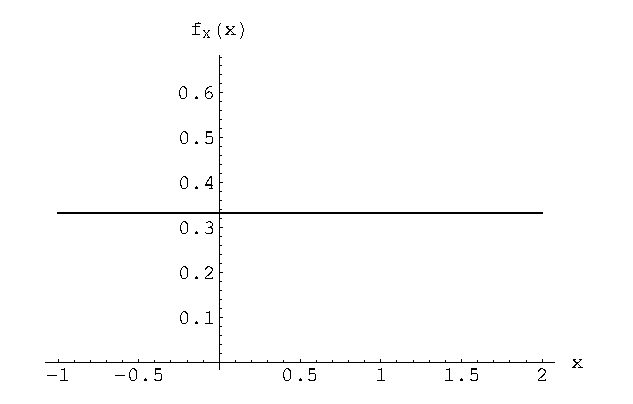
\includegraphics[scale=0.75]{densidaduniforme12}
&

       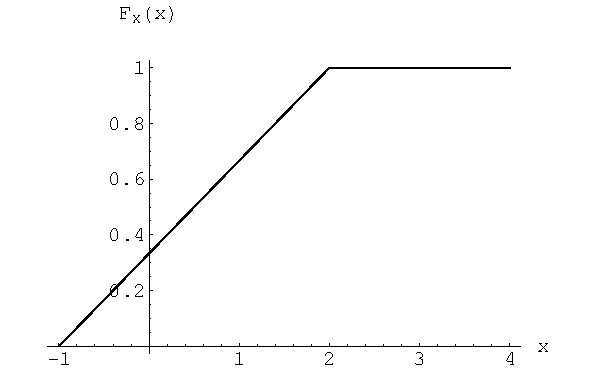
\includegraphics[scale=0.75]{distribucionuniforme12}\\ a) & b) \end{tabular}
\end{center}
       \caption{ Gráficas de la función de densidad (a)  y de la función de distribución (b) de una v.a. $U(-1,2)$.}
        \end{figure}%%%%%%%%  Sea $X$ una v.a. continua diremos que tiene distribución
%%%%%%%%          uniforme en el intervalo $(a,b)$ si su función de distribución
%%%%%%%%          es
%%%%%%%%          $$F_{X}(x)=\left\{\begin{array}{ll} 0 & \mbox{ si } x\leq a\\
%%%%%%%%          \frac{x-a}{b-a} & \mbox{ si } a\leq x\leq\\
%%%%%%%%          1 & \mbox{ si } b\leq x\end{array}\right.$$
%%%%%%%%
%%%%%%%%          $F$ es absolutamente continua y tiene por densidad:
%%%%%%%%         $$f_{X}(x)=\left\{\begin{array}{ll} \frac{1}{b-a} & \mbox{ si }
%%%%%%%%         a<x<b\\
%%%%%%%%         0 & \mbox{en el resto de casos}\end{array}\right.$$



\subsubsection{Cambio lineal v.a. uniforme}


Si $X$ sigue una distribución $U(a,b)$ entonces  $Z=\frac{x-a}{b-a}$ sigue una distribución $U(0,1)$.

En general si $d$ y $e$ son dos constantes reales  $T=d\cdot X+e$ sigue una ley $U(d\cdot a +e,d\cdot b +e)$  si $d>0$, cuando $d$ sea negativo $T$ sigue una ley 
$U(d\cdot b +e,d\cdot a +e)$. Las demostración se dejan como ejercicios.



\subsubsection{Resumen v.a con distribución uniforme, $U(a,b)$}

\scriptsize
\begin{tabular}{|c|c|c|c|c|}
\hline \begin{tabular}{c} Valores\\ admisibles.\end{tabular} & $f_{X}(x)$ & $F_X(x)=P(X\leq
X)=$ &
 $E(X)$ & $Var(X)$\\\hline & & & &\\
 $D_X=(a,b)$ & $\left\{\begin{array}{ll}
\frac{1}{b-a} & \mbox{si } a<x<b\\ 0  & \mbox{en cualquier otro caso}
\end{array}
\right.$  &  $\left\{\begin{array}{ll} 0 & \mbox{ si } x\leq a\\
          \frac{x-a}{b-a} & \mbox{ si } a\leq x\leq\\
          1 & \mbox{ si } b\leq x\end{array}\right.$
 & $\frac{a+b}{2}$ & $\frac{(b-a)^2}{12}$ \\& & & &\\ \hline
\end{tabular}

\normalsize



         \subsection{Distribución exponencial (exponencial negativa):}
         Supongamos que tenemos un proceso Poisson con parámetro
         $\lambda$ en una unidad de tiempo.

         Sea $t$ una cantidad de tiempo en u.t. entonces $N_{t}=$ número de
         eventos en el intervalo de tiempo $(0,t]$
         es una $Po(\lambda\cdot t)$. Consideremos la v.a.
         $T=$tiempo transcurrido entre dos eventos Poisson consecutivos.

         Sea $t>0$, entonces
         $$P(T>t)=P(\mbox{Cero eventos en el
         intervalo}(0,t])
         =P(N_{t}=0)=
         \frac{(\lambda t)^0}{0!} e^{-\lambda
         t}=e^{-\lambda t}.$$


         Tomando complementarios, la función de distribución de $T$ será

         $$F_{T}(t)=P(T\leq t)=\left\{\begin{array}{ll} 0 &\mbox{ si } t\leq 0\\
          1-P(T>t)=1-e^{-\lambda t}& \mbox{ si } t>0\end{array}\right.$$

         Entonces

         $$f_{T}(t)=\left\{\begin{array}{ll}
         \lambda e^{-\lambda t} & \mbox{ si }  t>0\\
         0 & \mbox{ si } t\leq 0
         \end{array}\right.$$

         La exponencial se denota por $Exp(\lambda)$

\subsubsection{Propiedad de la falta de memoria}

          Sea $X$  una v.a. $Exp(\lambda)$ entonces

          $$P(X>s+t/X>s)=P(X>t)\mbox{  para todo } s,t\in \R$$

          Toda v.a. absolutamente continua, que tome valores positivos
          y que verifique la propiedad de la falta de memoria es una v.a.
          exponencial.



\subsubsection{Resumen v.a con distribución exponencial, $Exp(\lambda)$}

Sea $X\equiv Exp(\lambda).$

\scriptsize
\begin{tabular}{|c|c|c|c|c|}
\hline \begin{tabular}{c} Valores\\ admisibles.\end{tabular} & $f_{X}(x)$ & $F_X(x)=P(X\leq
X)=$ &
 $E(X)$ & $Var(X)$\\\hline & & & &\\
 $D_X=(0,+\infty)$ & $\left\{\begin{array}{ll}
         \lambda e^{-\lambda x} & \mbox{ si }  x>0\\
         0 & \mbox{ si } x\leq 0
         \end{array}\right.$ &  $F_{X}(x)=P(X\leq x)=\left\{\begin{array}{ll} 0 &\mbox{si } x\leq 0\\
          1-e^{-\lambda x}& \mbox{si } x>0\end{array}\right.
$ & $\frac{1}{\lambda}$ & $\frac{1}{\lambda^2}$ \\& & & &\\ \hline
\end{tabular}

\normalsize




          \subsection{Distribución normal o Gaussiana}


          Diremos que una v.a. $X$ sigue una ley normal de parámetros
          $\mu$ y $\sigma^2$ y lo denotaremos por $N(\mu,\sigma^2)$
          si tiene por función de densidad

          $$f_{X}(x)=\frac{1}{\sqrt{2\pi}\sigma}
          e^{\frac{-(x-\mu)^2}{2\sigma^{2}}}\mbox{ para todo }x\in \RR$$

          La gráfica de esta función es la conocida campana de Gauss.

          La v.a. normal con $\mu=0$ y $\sigma=1$ recibe el nombre de
          normal estándar y se suele denotar por la letra $Z$.


%%%%%%%%          \textbf{Propiedad} Sea $X$ una v.a. $N(\mu,\sigma^2)$ y sea
%%%%%%%%          $f_{X}$ su función de densidad. Entonces:
%%%%%%%%          \vskip -1cm
%%%%%%%%          \begin{enumerate}[a)]
%%%%%%%%          \item Evidentemente $f_{X}$ verifica todas las pro\-pie\-da\-des de las
%%%%%%%%          funciones de densidad.
%%%%%%%%          \item $f_{X}(\mu-x)=f_{X}(\mu+x)$ es simétrica respecto de la recta
%%%%%%%%          $x=\mu$
%%%%%%%%          \item $f_{X}$ alcanza el máximo en $x=\mu$
%%%%%%%%         \item Si $F_{X}$ la función de distribución de $X$ entonces
%%%%%%%%         $F_{X}(\mu+x)=1-F_{X}(\mu-x)$. En par\-ti\-cu\-lar si $Z$ es una
%%%%%%%%         $N(0,1)$ entonces $F_{Z}(-x)=1-F_{Z}(x)$
%%%%%%%%         \item $Z=\frac{X-\mu}{\sigma}$ es una v.a. $N(0,1)$ y
%%%%%%%%              $X=\sigma Z+\mu$ es una $N(\mu,\sigma^{2})$ donde $Z$ es la
%%%%%%%%              normal estándar.
%%%%%%%%
%%%%%%%%          \end{enumerate}
%%%%%%%%



%%%%%%%%\section{La distribución normal o de Gauss}
%%%%%%%%
%%%%%%%% Diremos que una v.a. continua $X$ tiene
%%%%%%%%distribución normal con parámetros $\mu$ y  $\sigma^{2}$ a una variable aleatoria que tenga
%%%%%%%%por función de densidad :
%%%%%%%%$$f(x)={1\over{\sqrt{2\pi}\sigma}} {e\vphantom{A}}^{\left(-{1\over
%%%%%%%%2}{\left({x-\mu}\over{\sigma}\right)}^{2}\right)}$$



\begin{figure}[h]
\begin{center}
\begin{tabular}{cc}
 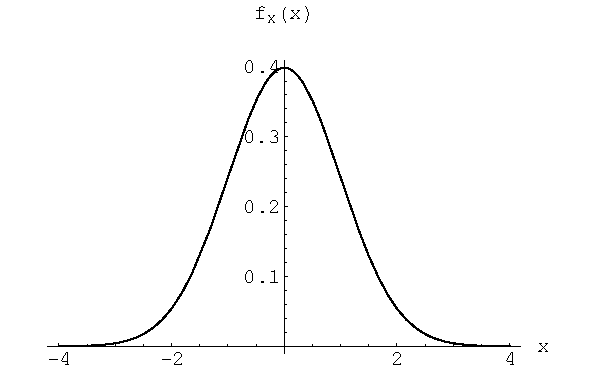
\includegraphics[scale=0.75]{densidadgaussiana}
&
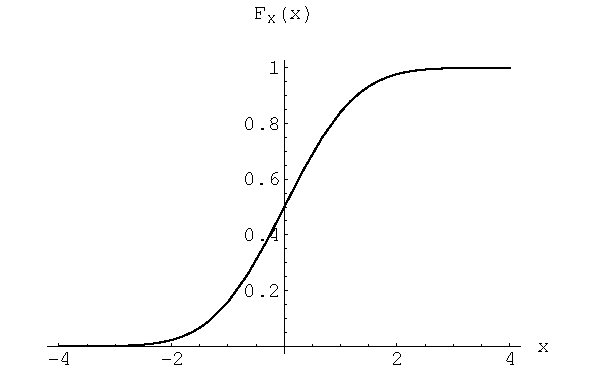
\includegraphics[scale=0.75]{distribuciongaussiana}\\ a) & b) \end{tabular}
\end{center}
       \caption{Gráficas de la función de densidad (a)  y de la  función de distribución (b) de una v.a. $N(0,1)$.}
        \end{figure}


%%%%%%%%\begin{figure}
%%%%%%%%\begin{center}
%%%%%%%%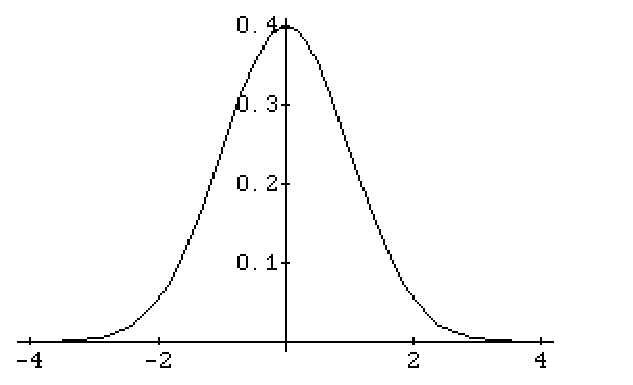
\includegraphics{normal.eps}
%%%%%%%%\end{center}
%%%%%%%%\caption{Curva de Gauss con $\mu=0$ y $\sigma=1$ }
%%%%%%%%\end{figure}



Su función de distribución es, como sabemos :
$$F(x)=\int_{-\infty}^{x} {1\over{\sqrt{2\pi}\sigma}}
{e\vphantom{A}}^{-{1\over 2}{\left({t-\mu}\over{\sigma}\right)}^{2}} dt$$

Que no tiene ninguna expresión algebraica ``decente''. Es por esta razón, y  por comodidad,
que esta función está tabulada.



Cuando una variable tiene distribución normal con parámetros $\mu,\sigma$ la denotamos por
$X\equiv N(\mu,\sigma^2)$


\subsubsection{Resumen v.a con distribución normal, $N(\mu,\sigma^2)$}

\scriptsize
\begin{tabular}{|c|c|c|c|c|}
\hline \begin{tabular}{c} Valores\\ admisibles.\end{tabular} & $f_{X}(x)$ & $F_X(x)=P(X\leq
X)=$ &
 $E(X)$ & $Var(X)$\\\hline & & & &\\
 $D_X=\RR$ & $=\frac{1}{\sqrt{2\pi}\sigma}
          e^{\frac{-(x-\mu)^2}{2\sigma^{2}}}\mbox{ para todo }x\in \R$ & Tabulada la
          $N(0,1)$ & $\mu$ & $\sigma^2$ \\& & & &\\ \hline
\end{tabular}
\normalsize



\subsubsection{Propiedades de la distribución normal.} La función de densidad de la
distribución normal tiene las siguientes propiedades:
\begin{enumerate}[a)]
\item $f$ es continua
\item $\int_{-\infty}^{+\infty} {1\over{\sqrt{2\pi}\sigma}} {e\vphantom{A}}^{-{1\over
2}{\left({x-\mu}\over{\sigma}\right)}^{2}} dx =1$ ( propiedad de todas las densidades).
\item $f(\mu+x)=f(\mu-x)$ y $F(x+\mu)=1-F(\mu-x)$ para todo $x\in \cal{R}$
\item $\lim\limits_{x\to+\infty}f(x)=\lim\limits_{x\to-\infty}f(x)=0$
es decir tiene asíntota horizontal a derecha e izquierda.
\item $f$ es estrictamente creciente si $x<\mu$ y decreciente si $x>\mu$.
\item Alcanza el máximo en $x=\mu$ y en este punto vale $f(\mu)=\frac{1}{\sqrt{2\pi}\sigma}$
\item Tiene dos puntos de inflexión en $x=\mu+\sigma$ y en $x=\mu-\sigma$.
\end{enumerate}


\subsubsection{Transformaciones lineales de variables aleatorias normales}

\begin{proposition} Sea $X\equiv N(\mu,\sigma^2)$  entonces la variable $Y=a X+b$ con
$a\not=0,b\in\cal{R}$ tiene distribución $N(a\mu+b, a^2 \sigma^2)$

En particular si  $X\equiv N(\mu,\sigma^2)$, tomando $a=\frac{1}{\sigma}$ y $b=
\frac{-\mu}{\sigma}$ la v.a. $Z={{X-\mu}\over {\sigma}}$ se distribuye $N(0,1)$.

Esta propiedad es muy importante, ya que utilizándola sólo necesitaremos tabular la
$N(0,1)$. A la función de distribución de una $Z\equiv N(0,1)$ la llamaremos $F_Z$  y a una
normal $N(0,1)$  se le denomina normal estándar. Por lo tanto si
$F_X(x)=F_Z(\frac{x-\mu}{\sigma})$.
\end{proposition}

La propiedad siguiente se desprende de las propiedades generales de una normal y nos será
muy útil en los cálculos de probabilidades de una normal.

\textbf{Propiedad} Si $Z\equiv N((0,1)$ entonces $F_{Z}(x)=1-F_{Z}(-x)$.

\begin{example} Sea $Z\equiv N(0,1)$  Calcular :
\begin{enumerate}[a)]
\item Dado $\delta>0$, $P(-\delta\leq Z \leq
\delta)=F_{Z}(\delta)-F_{Z}(-\delta)=F_Z(3)-(1-F_Z(\delta))=2 F_Z(\delta)-1$
\item $P(-4\leq Z \leq 4)=F_{Z}(4)-F_{Z}(-4)=2 F_Z(4)-1$
\item $P(-2\leq Z \leq 2)=F_{Z}(2)-F_{Z}(-2)=2 F_Z(2)-1$
\item $P(Z\leq -2)=F_Z(-2)=1-F_Z(2)$
\item $P( Z \leq 2)=F_{Z}(2)$
\item $P( Z \geq 2)=1-P(Z<2)=1-F_{Z}(2)$
\item $P( Z > 2)=1-P(Z\leq 2)=1-F_{Z}(2)$
\item $P( Z = 2)=0$
\item $P( Z \geq -2)=1-P(Z< -2)=1-F_{Z}(-2)=1-(1-F_Z(2))=F_Z(2).$
\end{enumerate}
\end{example}
    Resumiendo podemos utilizar las siguientes propiedades, $X\equiv N(\mu,\sigma)$
    \begin{itemize}
    \item  $Z$ es su variable tipificada, es decir,
    $Z=\frac{X-\mu}{\sigma}\equiv N(0,1)$ entonces:

    $$P(X\leq x)=P(\frac{X-\mu}{\sigma}\leq
    \frac{x-\mu}{\sigma})=F_{Z}(\frac{x-\mu}{\sigma})$$

   \item  Cuando tengamos un intervalo
    $$P(a<X<b)=P(\frac{a-\mu}{\sigma}<\frac{X-\mu}{\sigma}<\frac{b-\mu}{\sigma})=$$

    $$=P(\frac{a-\mu}{\sigma}<Z<\frac{b-\mu}{\sigma})=F_{Z}(\frac{b-\mu}{\sigma})-
    F_{Z}(\frac{a-\mu}{\sigma})$$
    \item Si $\delta>0$ $P(\mu-\delta\leq X \leq
\mu+\delta)=2 F_Z(\frac{\delta}{\sigma})-1$
\end{itemize}


    \begin{example}Sea $X$ una normal com media $2$ y varianza $4$, entonces
    \begin{enumerate}[a)]
\item  $P(1< X< 2)= P(\frac{1-2}{2}<\frac{X-2}{2}<\frac{2-2}{2})=
    P(\frac{-1}{2}<Z<0)=F_{Z}(0)-F_{Z}(-0.5)=\frac{1}{2}-1+F_{Z}(0.5).$
    \item $P(X>3)=P(\frac{X-2}{2}>\frac{3-2}{2})=
    P(Z>0.5)=1-F_{Z}(0.5).$
    \end{enumerate}
\end{example}
